\section{EVALUACIÓN}
% Explicar el conjunto de validació cruzada
% Mostrar métricas de aprendizaje
% Listar resultados de predicción
% Mostrar los clusters encontrados por k means
% Justificar el uso de 4 clusters
Se analizan las curvas de aprendizaje para cada modelo usando Adam como optimizador.

\subsection{DRIVENET}
Para la red de conducción se tiene la curva dada en la figura \ref{drivenetcurve} de un total de 30 iteraciones, con parámetros $\alpha=0.001$, $\beta_1=0.9$, $\beta_2=0.999$. De estos resultados se decidió realizar pruebas entre la iteración 24 y 30, se tomaron los parámetros de la epoch 24 con errores cuadráticos medios de 0.00051 para el conjunto de entrenamiento y 0.00088 para el conjunto de validación.

\begin{figure}[H]
	\centering
	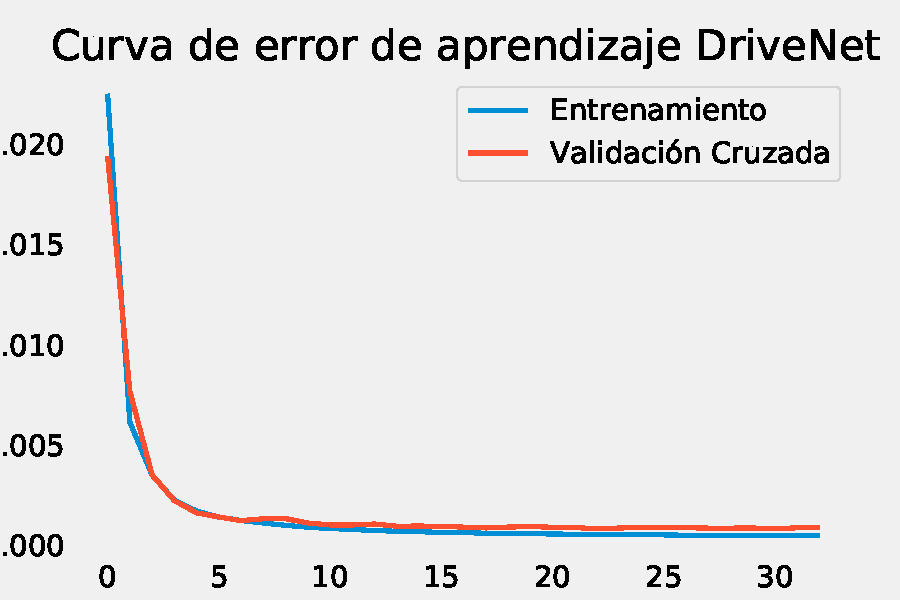
\includegraphics[scale=0.5]{imagenes/DriveNetCurve}
	\caption[Errores de entrenamiento y validación de la DriveNet]{errores de entrenamiento y validación de la DriveNet}
	\label{drivenetcurve}
\end{figure}

\subsection{DEPTHNET}
Para la red de profundidad se tiene la curva dada en la figura \ref{depthnetcurve} de un total de 24 iteraciones, con parámetros $\alpha=0.01$, $\beta_1=0.9$, $\beta_2=0.999$.

\begin{figure}[H]
	\centering
	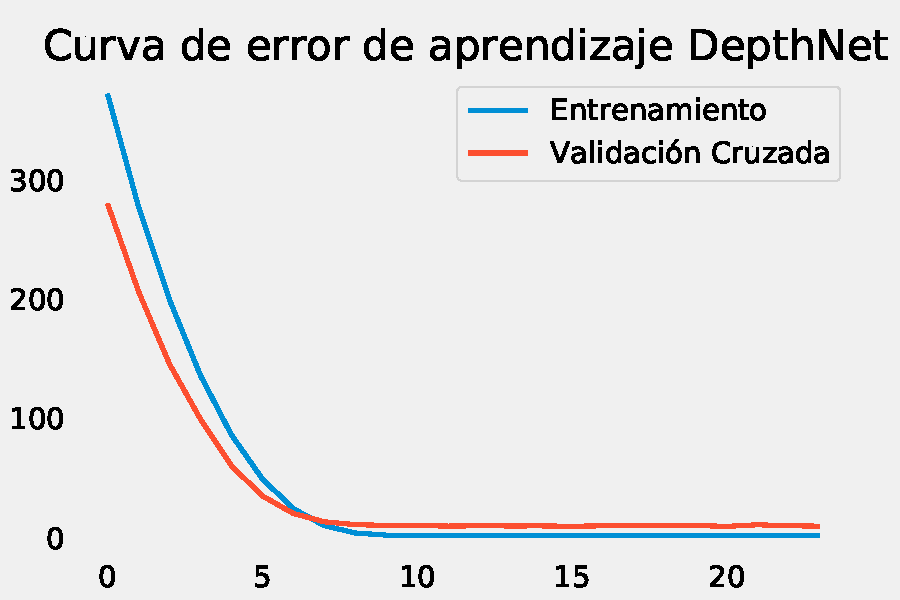
\includegraphics[scale=0.5]{imagenes/DepthNetCurve}
	\caption[Errores de entrenamiento y validación de la DepthNet]{errores de entrenamiento y validación de la DepthNet}
	\label{depthnetcurve}
\end{figure}

De estos resultados se eligieron los parámetros de la iteración 20 con errores cuadráticos medios de 1.30575 para el conjunto de entrenamiento y 9.267 para el conjunto de validación.

Es importante notar que no se tomaron los parámetros de alguna iteración que distara poco del error de entrenamiento, sino de la iteración en la que se tenía el menor error de validación durante el entrenamiento.

\subsection{SEMSEGNET}
Para la red de segmentación semántica se tiene la curva dada en la figura \ref{semsegnetcurve} de un total de 7 iteraciones, ya que esta era la más costosa de computar, con los mismos parámetros que la DriveNet.

\begin{figure}[H]
	\centering
	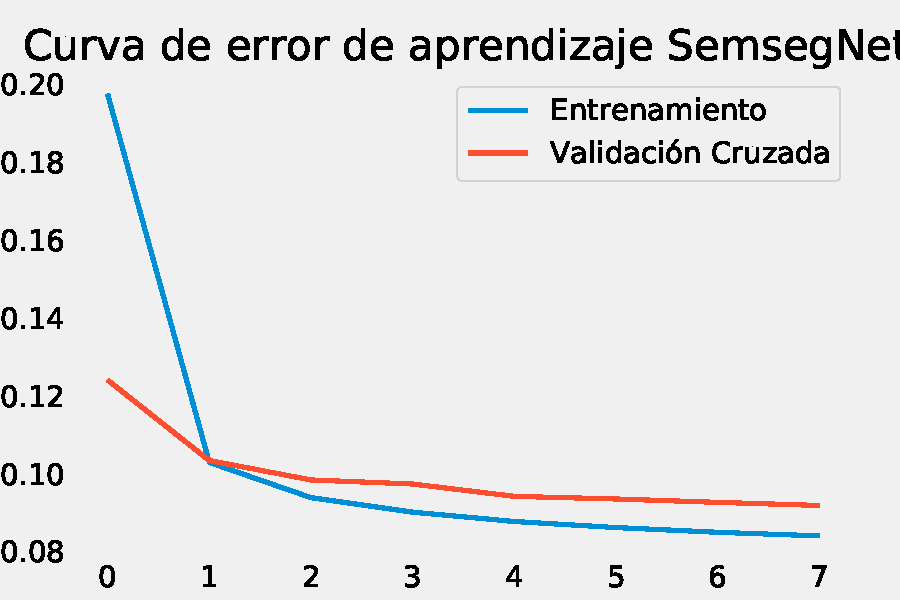
\includegraphics[scale=0.5]{imagenes/SemsegNetCurve}
	\caption[Errores de entrenamiento y validación de la SemsegNet]{errores de entrenamiento y validación de la SemsegNet}
	\label{semsegnetcurve}
\end{figure}

De estos resultados se eligieron los parámetros de la iteración 7 con errores del tipo mean log softmax 2D de 0.08396 para el conjunto de entrenamiento y 0.09178 para el conjunto de validación.

Al igual que para la red de profundidad se eligieron los parámetros con el menor error en el conjunto de validación cruzada.

\subsection{CENTROIDES K-MEANS}
Finalmente se evalúa que la decisión sea correcta para el número de centroides en el algoritmo KMEans, debido a que el espacio de color RGB se puede representar como 3 dimensiones espaciales, se analizó gráficamente el desempeño del algoritmo, se decidió que 4 centroides era la mejor cantidad para la tarea de cuantificación digitalización del color.

Observando la figura \ref{colorspace}, se nota que de los cuatro centroides señalizados con figuras distintas de esferas y de color azul, dos de ellos están en el punto de mayor aglomeración que son los píxeles de colores oscuros del borde del semáforo, mientras que los otros dos están en los puntos más intensos del color rojo o verde y en el punto de combinación entre dos colores, blanco para el caso verde-azul y amarillo para rojo-verde.

\begin{figure}[H]
	\centering
	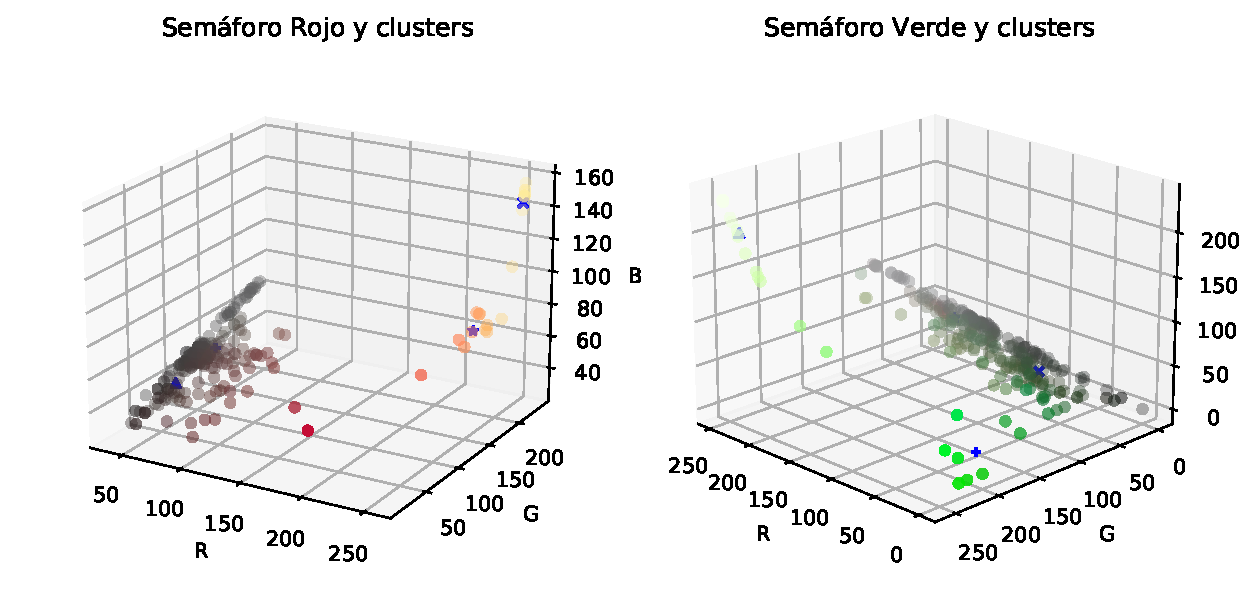
\includegraphics[scale=0.65]{imagenes/sign_3d}
	\caption[Espacios de color y centroides para dos semáforos distintos]{espacios de color y centroides para dos semáforos distintos}
	\label{colorspace}
\end{figure}